\section{Compressed Sensing Image Reconstruction for MeerKAT} \label{intro}
Image reconstruction problems arise in a variety of fields. Real-world imaging instruments measure noisy, corrupted data. Reconstruction algorithms are tasked with removing the corruption and finding the observed image. The theory of Compressed Sensing\cite{candes2006robust, donoho2006compressed} gives a framework for analysis and design of reconstruction algorithms, and we apply it to the large scale reconstruction problem of the new MeerKAT Radio Interferometer.

The MeerKAT Interferometer does not measure pixels of the image directly. Instead, it measures a noisy, incomplete set of Fourier Components, which can take up several hundred gigabytes of disk space. Multiple images fit the measurements, and the reconstruction algorithm has to find the observed image from a large set of candidates. This data volume forces the reconstruction to be distributed on multiple machines. The state-of-the-art approach is based on CLEAN\cite{rich2008multi, rau2011multi} and its new implementation WSCLEAN\cite{offringa2014wsclean} is the go-to software package for MeerKAT reconstructions.

Recently, new algorithms based on Compressed Sensing created super-resolved images of real-world observations \cite{girard2015sparse, dabbech2018cygnus}. They have the potential to increase the effective accuracy of the instrument. However they come with higher runtime costs compared to WSCLEAN. In Radio astronomy, CLEAN and Compressed Sensing algorithms use the non-uniform FFT approximation\cite{kunisnonequispaced, pratley2017robust} to cycle between measurements and image space. Compressed Sensing algorithms need more cycles to converge, which is one source of the higher runtime costs. 

In this project we investigate if the runtime costs of Compressed Sensing Reconstructions can be reduced by replacing the non-uniform FFT. We created a proof-of-concept algorithm which does not need the non-uniform FFT during optimization. Instead, we use the direct Fourier Transform which potentially leads to a distributable Compressed Sensing algorithm. Sadly, our new approach cannot reduce the runtime costs of large scale reconstructions.

We demonstrate our algorithms and its current limitations. The rest of this article is structured as the following: We begin by introducing the basic image reconstruction problem in radio interferometry. We show the Major Cycle architecture for reconstruction algorithms, which is derived from the non-uniform FFT.  Section \ref{meerkat} introduces the difficulties of imaging MeerKAT data. We  move towards alternatives to the non-uniform FFT in section \ref{killmajor}. In the following sections \ref{cd}, \ref{results} and \ref{scale} we introduce our Compressed Sensing algorithm, show the reconstruction quality on simulated MeerKAT data and extrapolate the runtime costs on a real world MeerKAT measurement.


\subsection{The Basic Reconstruction Problem of Radio Interferometers}\label{intro:basic}
We start with a simplified measurement equation for Radio Interferometers, \eqref{intro:measurement}. An interferometer measures an incomplete set of Fourier Components $V$ (called Visibilities in Radio Astronomy) from the sky image $I$ at position $x$ and $y$. We want to reconstruct the image $I$, while the instrument measures $V$ in a noisy environment. Since the term $e^{2 \pi i (ux+vy)}$ is the Fourier Transform, the image can be calculated from the Visibilities by the inverse Fourier Transform.

\begin{equation}\label{intro:measurement}
V(u, v) = \int\int I(x, y) e^{2 \pi i (ux+vy)} \: dx \: dy
\end{equation}

However, the Visibilities are incomplete and noisy. The inverse Fourier Transform does not give us the observed image, but a corrupted "dirty" image.  It introduces structures in the dirty image which were not observed. The incomplete Visibility coverage effectively convolves the observed image with a Point Spread Function. A reconstruction algorithm has to decide which structures were truly observed, and which are due to noise and incomplete Visibility coverage. In the framework of Compressed Sensing, this leads us to a minimization problem with the following objective function:

\begin{equation}\label{intro:cs}
\underset{x}{minimize} \: \left \| V - Fx \right \|_2^2 + \lambda \left \| P(x) \right \|_1
\end{equation}

The objective \eqref{intro:cs} is split into two terms, the data and regularization term. The data term forces the reconstructed image to be as close to the measurements as possible, while the regularization term penalises unlikely images. Overall, we try to find the optimal image, which is as close to the Visibilities as possible, but also has the smallest regularization penalty according to some prior function $P()$. The parameter $\lambda$ weights the trade-off between the data and regularization term. The theory of Compressed Sensing states that if our prior function $P()$ models the observed image well, we are virtually guaranteed to find it at the minimum of our objective function \eqref{intro:cs}.

The question is, what is a good prior? This depends on the image content. For example if our Interferometer measures an image containing only stars (called point-sources), our observed image will only contain a non-zero pixels at the locations of the stars. In this case, the $L1$ norm\footnote{simply the absolute value of the image, $abs(x)$} is a good prior. It will force the reconstruction to have as few non-zero pixels as possible, and we are likely to find the truly observed image at the minimum of \eqref{intro:cs}.

In theoretical terms, the reconstruction problem for Radio Interferometry boils down to finding a good prior function $P()$, and an efficient optimization algorithm to minimize \eqref{intro:cs}. In the real-world, we have millions of pixels and several billions of Visibilities in a single reconstruction for MeerKAT. The Fourier Transform Matrix $F$ with the size of Visibilities times pixels becomes expensive to either compute or keep in memory. Also, we cannot use the Fast Fourier Transform, because the interferometer measures an incomplete and non-uniformly sampled set of Visibilities. For an efficient reconstruction algorithm, we need to handle the Fourier Transform in an efficient manner.

The large Fourier Transform matrix is common for image reconstructions in Radio Astronomy. MeerKAT just poses the same problem on an even larger scale.
State-of-the-art reconstructions deal with the large $F$ by using the non-uniform FFT approximation.

\subsection{The non-uniform FFT and the Major Cycle}\label{intro:nufft}
In Radio Astronomy, state-of-the-art reconstruction algorithms use the non-uniform FFT to approximate the Fourier Transform. They use the approximation to continually cycle between Visibility and image space during reconstruction. CLEAN calls this the Major Cycle, which is used for virtually every CLEAN reconstruction of Radio Interferometers. 

\begin{equation}\label{intro:clean}
\underset{x}{minimize} \: \left \|  I_{Dirty} - x \star PSF \right \|_2^2 + \lambda \left \| x \right \|_1 \quad, \quad I_{Dirty} = \hat{F}^{-1} V
\end{equation}

%The CLEAN algorithm can work outside the Major Cycle and the non-uniform FFT. But for the large Fourier Matrix $F$ of interferometers, the non-uniform FFT generally leads to lower runtime costs.
In a Major Cycle, the Visibilities get transformed into image space, CLEAN deconvolves the image with the $PSF$, and the residual image gets transformed back into Visibilities as shown in figure \ref{intro:major}. It minimizes roughly the objective \eqref{intro:clean}\footnote{ In reality CLEAN uses a number of heuristics which are hard to formalize. This objective is a mere approximation to highlight its properties in our context.}. As we will see, continually cycling between Visibility an image space has advantages, which current Compressed Sensing algorithms inherit by using the non-uniform FFT. We show the advantages of the non-uniform FFT at the example of CLEAN and the Major Cycle architecture, and discuss the implications for Compressed Sensing algorithms.


\begin{figure}[h]
	\centering
	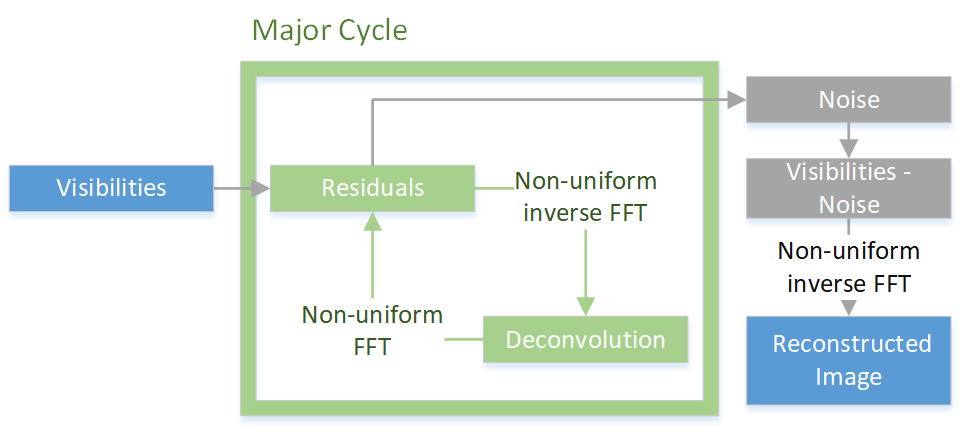
\includegraphics[width=0.80\linewidth]{./chapters/01.intro/Major-Minor.png}
	\caption{The Major Cycle Framework}
	\label{intro:major}
\end{figure}

In each Major Cycle of figure \ref{intro:major}, the residual Visibilities get transformed by the non-uniform FFT, CLEAN approximates the deconvolution, and the new residual image gets transformed back to Visibilities. Over several Major Cycles the error from the non-uniform FFT and from the CLEAN deconvolutions get minimized. In a sense, the Major Cycle is a simple optimization algorithm for two different errors. This lets CLEAN approximate the deconvolution with a constant $PSF$. The $PSF$ for Radio interferometer reconstructions varies over the image. With the Major Cycle, CLEAN can reduce the error of the constant $PSF$ introduced of the previous cycle, and lead to an overall more accurate reconstruction.

State-of-the art Compressed Sensing algorithms also use the non-uniform FFT and inherit similar advantages from the Major Cycle. The error of the Fourier approximation gets continually reduced over several cycles. More complex measurement equations have been incorporated with the non-uniform FFT in mind, and work similar for both CLEAN and Compressed Sensing based algorithms. 


 







